\documentclass[]{beamer}
\usetheme{KUL}
\usepackage{multirow}
\usepackage{multicol}
\usepackage{tikz}
\usepackage{ulem}
\usepackage{siunitx}
\newcommand\itemS{\item[\textbf{\S}]}
\definecolor{darkgreen}{rgb}{0,0.598,0.199}
\usepackage{times} % set font on times new roman
\usepackage{eurosym} % package for Euro sign
\usepackage{lineno}   % package for line numbering
\usepackage{hyperref} % this is for url links
\usepackage{subcaption}  % this package enables one to put several figures next to each other
\usepackage{textcomp}
\usepackage{setspace}
\usepackage{gensymb}
\newenvironment{figure*}%
{\begin{figure}}
{\end{figure}}
%----------------------------------
% Fill in the essential Information
%----------------------------------

\title[Individualizaci\'on de filamentos mediante optimizaci\'on]{Defensa de Tesis: Individualizaci\'on de filamentos en una red mediante optimizaci\'on}
%\subtitle{\ldots a subtitle}
\author[L.\ Pizarro]{Leonardo Pizarro} % between [] is short name, between {} is long name
\date{\today} % Here you can also just type something, e.g. October 10, 2017
\institute[DCC - FCFM - UChile]{Magister en Ciencias de la Computación\\Facultad de Ciencias F\'isicas y Matem\'aticas\\ Departmento de Ciencias de la Computaci\'on \\ Universidad de Chile}

%----------------------------------
% ACTUAL PRESENTATION STARTS HERE
%----------------------------------

\begin{document}

% TITEL PAGE	
	{
		\setbeamertemplate{headline}{} %define local, empty header for title page
		\setbeamertemplate{footline}{} %define local, empty footer for title page
		\maketitle
	}
	\addtocounter{framenumber}{-1} % We don't count the title page

\begin{frame}
\frametitle{Contenidos} 
\tableofcontents
\end{frame}

\section{Motivaci\'on y antecedentes}
% [allowframebreaks] para dividir en multiples frames
\begin{frame}{Que es un filamento?}
    \begin{columns}
    \begin{column}{0.32\textwidth}
        \begin{itemize}
            \item Estructuras alargadas con diferentes propiedades
            \item Observaci\'on de Microscop\'ia
            \begin{itemize}
            \small
                \item Ruido
                \item Resoluci\'on
            \end{itemize}
        \end{itemize}
    \end{column}
    \begin{column}{0.68\textwidth}
        \begin{figure*}[h]
          \centering
            \begin{subfigure}[t]{0.48\textwidth}
            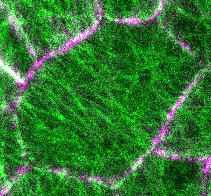
\includegraphics[height=1.2in]{Pictures/small_MT.jpg}
            \end{subfigure}
            ~ 
            \begin{subfigure}[t]{0.48\textwidth}
            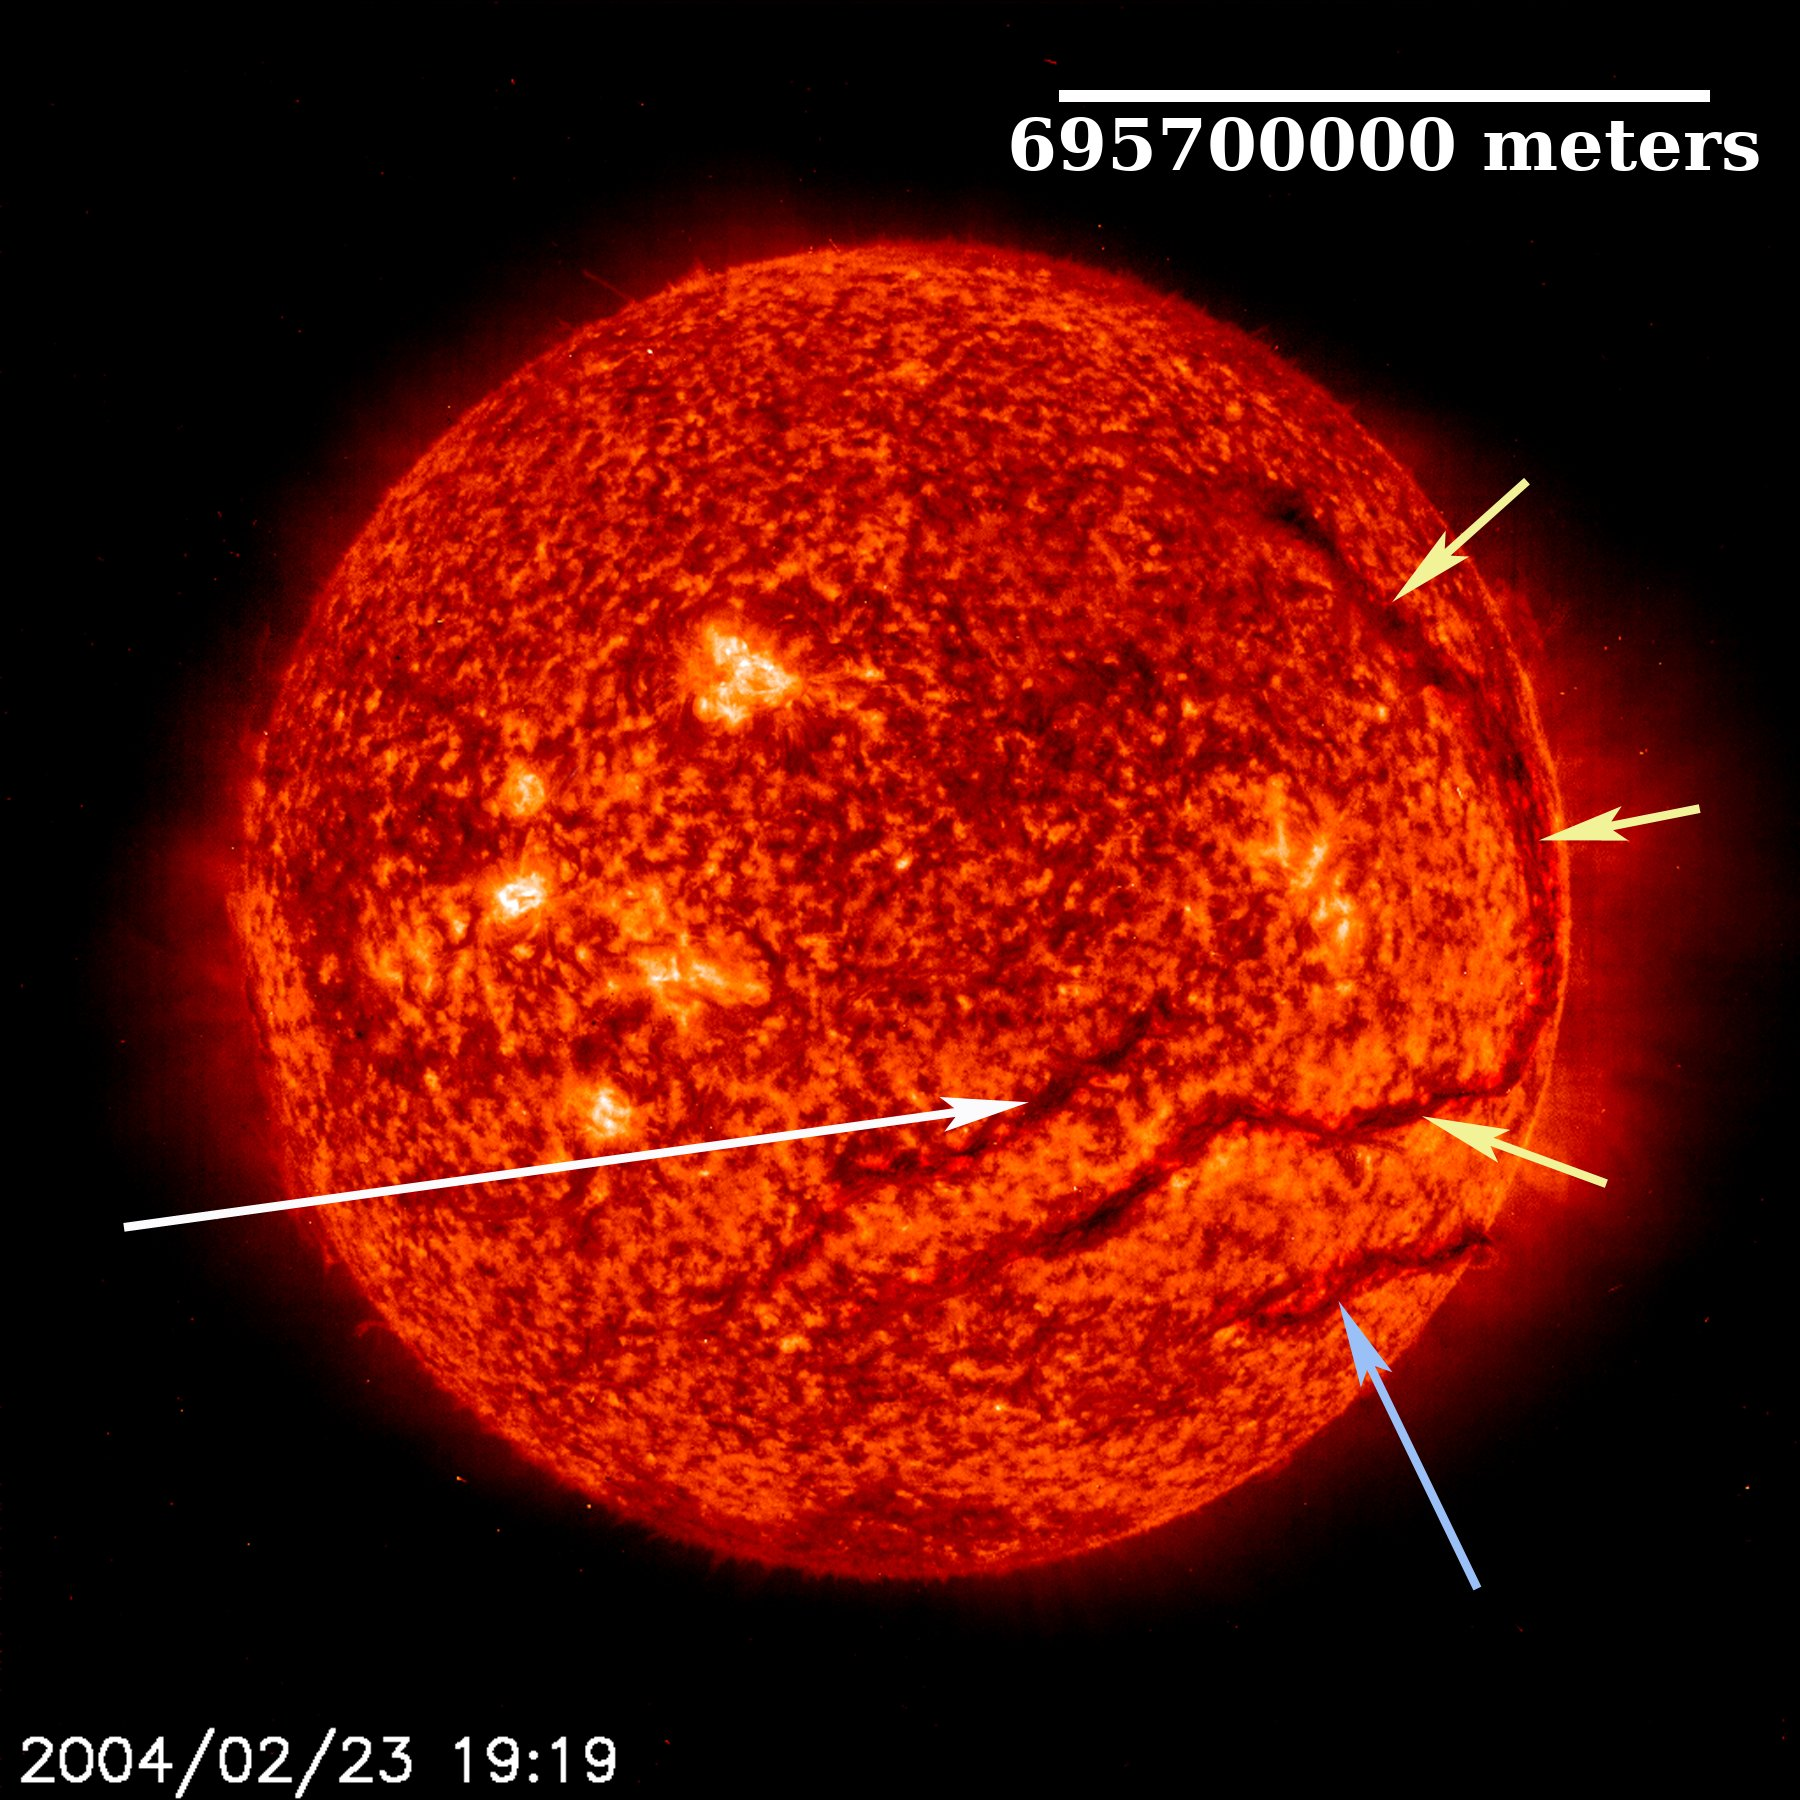
\includegraphics[height=1.2in]{Pictures/sun_filament.jpg}
            \end{subfigure}
            \vspace{0.5cm}
             \begin{subfigure}[t]{\textwidth}
             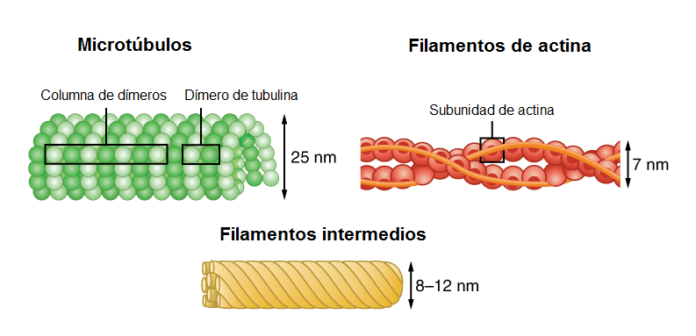
\includegraphics[height=1.2in]{Pictures/citoesqueletoo-min.png}
            \end{subfigure}
    
        \end{figure*}
    \end{column}
\end{columns}
\end{frame}

\begin{frame}{Varias soluciones posibles}
  \begin{columns}
    \begin{column}{0.6\textwidth}
    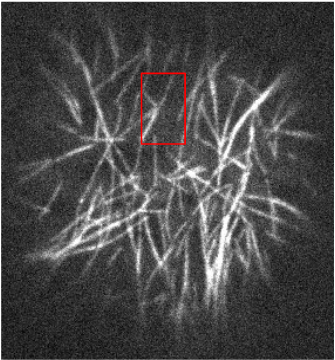
\includegraphics[scale=0.5]{Pictures/NoConsenso.png}
    \end{column}
    \begin{column}{0.2\textwidth}
    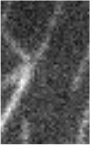
\includegraphics[scale=0.5]{Pictures/NoConsenso2.png}
    \end{column}
    \begin{column}{0.2\textwidth}
    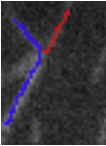
\includegraphics[scale=0.5]{Pictures/NoConsenso3.png}
    \vspace{0.5cm}
    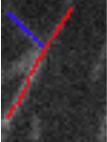
\includegraphics[scale=0.5]{Pictures/NoConsenso4.png}
    \end{column}
\end{columns}
\end{frame}

\begin{frame}{Hip\'otesis y Objetivo General}
\begin{itemize}
    \item Hip\'otesis:
    \vspace{1cm}
    \item Objetivo General
\end{itemize}
    
\end{frame}

\begin{frame}{Objetivos Espec\'ificos}
\begin{itemize}
    \item A
    \item B
    \item C
    \item D
\end{itemize}
    
\end{frame}

\subsection{Enfoques en la literatura}
\begin{frame}{M\'etodos basados en:}
    \begin{itemize}
        \item Vision por Computador
        \item Optimizaci\'on
        \begin{itemize}
            \item Metaheur\'istica ACO
        \end{itemize}
    \end{itemize}
\end{frame}


\subsection{Metaheur\'istica ACO}

\section{Algoritmo Propuesto}
\subsection{Inicializaci\'on ACO}
\subsection{Construcci\'on de Soluciones}
\subsection{Anti-Feromonas}
\subsection{M\'etodo de b\'usqueda no local}

\section{Resultados}
\begin{frame}{Metodolog\'ia}
\begin{itemize}
    \item 5 Iteraciones promediadas, con distinta semillas
\end{itemize}
    
\end{frame}
\begin{frame}{Im\'agenes Sint\'eticas}
    
\end{frame}
\begin{frame}{Microt\'ubulos}
    
\end{frame}

\begin{frame}{Neuronas de rat\'on}

\end{frame}

\section{Conclusiones}
\begin{frame}{Conclusiones}
    \begin{itemize}
        \item A
    \end{itemize}
\end{frame}

\end{document}